\documentclass[twoside]{book}

% Packages required by doxygen
\usepackage{fixltx2e}
\usepackage{calc}
\usepackage{doxygen}
\usepackage[export]{adjustbox} % also loads graphicx
\usepackage{graphicx}
\usepackage[utf8]{inputenc}
\usepackage{makeidx}
\usepackage{multicol}
\usepackage{multirow}
\PassOptionsToPackage{warn}{textcomp}
\usepackage{textcomp}
\usepackage[nointegrals]{wasysym}
\usepackage[table]{xcolor}

% Font selection
\usepackage[T1]{fontenc}
\usepackage[scaled=.90]{helvet}
\usepackage{courier}
\usepackage{amssymb}
\usepackage{sectsty}
\renewcommand{\familydefault}{\sfdefault}
\allsectionsfont{%
  \fontseries{bc}\selectfont%
  \color{darkgray}%
}
\renewcommand{\DoxyLabelFont}{%
  \fontseries{bc}\selectfont%
  \color{darkgray}%
}
\newcommand{\+}{\discretionary{\mbox{\scriptsize$\hookleftarrow$}}{}{}}

% Page & text layout
\usepackage{geometry}
\geometry{%
  a4paper,%
  top=2.5cm,%
  bottom=2.5cm,%
  left=2.5cm,%
  right=2.5cm%
}
\tolerance=750
\hfuzz=15pt
\hbadness=750
\setlength{\emergencystretch}{15pt}
\setlength{\parindent}{0cm}
\setlength{\parskip}{3ex plus 2ex minus 2ex}
\makeatletter
\renewcommand{\paragraph}{%
  \@startsection{paragraph}{4}{0ex}{-1.0ex}{1.0ex}{%
    \normalfont\normalsize\bfseries\SS@parafont%
  }%
}
\renewcommand{\subparagraph}{%
  \@startsection{subparagraph}{5}{0ex}{-1.0ex}{1.0ex}{%
    \normalfont\normalsize\bfseries\SS@subparafont%
  }%
}
\makeatother

% Headers & footers
\usepackage{fancyhdr}
\pagestyle{fancyplain}
\fancyhead[LE]{\fancyplain{}{\bfseries\thepage}}
\fancyhead[CE]{\fancyplain{}{}}
\fancyhead[RE]{\fancyplain{}{\bfseries\leftmark}}
\fancyhead[LO]{\fancyplain{}{\bfseries\rightmark}}
\fancyhead[CO]{\fancyplain{}{}}
\fancyhead[RO]{\fancyplain{}{\bfseries\thepage}}
\fancyfoot[LE]{\fancyplain{}{}}
\fancyfoot[CE]{\fancyplain{}{}}
\fancyfoot[RE]{\fancyplain{}{\bfseries\scriptsize Generated by Doxygen }}
\fancyfoot[LO]{\fancyplain{}{\bfseries\scriptsize Generated by Doxygen }}
\fancyfoot[CO]{\fancyplain{}{}}
\fancyfoot[RO]{\fancyplain{}{}}
\renewcommand{\footrulewidth}{0.4pt}
\renewcommand{\chaptermark}[1]{%
  \markboth{#1}{}%
}
\renewcommand{\sectionmark}[1]{%
  \markright{\thesection\ #1}%
}

% Indices & bibliography
\usepackage{natbib}
\usepackage[titles]{tocloft}
\setcounter{tocdepth}{3}
\setcounter{secnumdepth}{5}
\makeindex

% Hyperlinks (required, but should be loaded last)
\usepackage{ifpdf}
\ifpdf
  \usepackage[pdftex,pagebackref=true]{hyperref}
\else
  \usepackage[ps2pdf,pagebackref=true]{hyperref}
\fi
\hypersetup{%
  colorlinks=true,%
  linkcolor=blue,%
  citecolor=blue,%
  unicode%
}

% Custom commands
\newcommand{\clearemptydoublepage}{%
  \newpage{\pagestyle{empty}\cleardoublepage}%
}

\usepackage{caption}
\captionsetup{labelsep=space,justification=centering,font={bf},singlelinecheck=off,skip=4pt,position=top}

%===== C O N T E N T S =====

\begin{document}

% Titlepage & ToC
\hypersetup{pageanchor=false,
             bookmarksnumbered=true,
             pdfencoding=unicode
            }
\pagenumbering{alph}
\begin{titlepage}
\vspace*{7cm}
\begin{center}%
{\Large N\+E\+D\+I\+SS\+: Network Diffusion and Synchronization Simulator }\\
\vspace*{1cm}
{\large Generated by Doxygen 1.8.13}\\
\end{center}
\end{titlepage}
\clearemptydoublepage
\pagenumbering{roman}
\tableofcontents
\clearemptydoublepage
\pagenumbering{arabic}
\hypersetup{pageanchor=true}

%--- Begin generated contents ---
\chapter{G\+R\+A\+P\+H\+V\+IZ}
\label{md_graphic_GRAPHVIZ}
\Hypertarget{md_graphic_GRAPHVIZ}

\begin{DoxyItemize}
\item manual for graphviz engines\+: \href{https://graphviz.org/docs/layouts/}{\tt https\+://graphviz.\+org/docs/layouts/}
\item summary of graphviz here-\/relevant engines\+: circo for ring,clique,smallworld, patchwork for grids, fdp and sfdp try them. sfdp for huges. 
\end{DoxyItemize}
\chapter{R\+E\+A\+D\+ME}
\label{md_README}
\Hypertarget{md_README}
\begin{center}\section*{{\bfseries V 1.\+0.\+0 is ready!}}\end{center} 

\begin{center} {\itshape (Decent documentation coming soon!)}\end{center}  



\begin{center}{\bfseries How to run}\end{center} 

{\itshape Just configure the simulation via {\ttfamily simulation.\+conf.\+sh} and execute the desired script}

1) {\ttfamily run.\+sh} runs the program in whichever mode was specified in the configuration file 2) {\ttfamily produce\+\_\+graphical\+\_\+simulation.\+sh} runs the program in simulation mode and produces a graphical simulation 4) {\ttfamily run\+\_\+debugxterm.\+sh} runs with gdb and displays each processor in a different console 5) {\ttfamily run\+\_\+pipe.\+sh} runs and pipes the output to a txt file 6) {\ttfamily run\+\_\+valgrind.\+sh} runs and produces a valgrind report 7) {\ttfamily run\+\_\+time.\+sh} runs nonverbose and computes the execution time

The configuration file allows the following to be specified\+:


\begin{DoxyItemize}
\item E\+Q\+N\+U\+M\+B\+ER\+: {\ttfamily \{0,1\}} indexes one of the O\+D\+Es described below. Currently {\ttfamily 0} for 1D linear and {\ttfamily 1} for Noiseless Kuramoto.
\item S\+O\+L\+V\+ER\+: {\ttfamily \{0,1\}} indexes the solver. {\ttfamily 0} for the Euler method and {\ttfamily 1} for Runge Kutta.
\item S\+O\+L\+V\+E\+R\+D\+E\+P\+TH\+: {\ttfamily \{1,2,3,4\}} is the depth used in Euler\textquotesingle{}s method. A depth of i with i$>$1 requires the (i-\/1)-\/th derivative of the Equation\textquotesingle{}s field to be implemented.
\item K1, K2, K3, K4\+: {\ttfamily \mbox{[}0,1\mbox{]}} are the weights to apply to each of the Runge Kutta terms.
\item T\+O\+P\+O\+L\+O\+GY\+: {\ttfamily \{0,1,2,3\}} indexes the topology. Currently {\ttfamily 0} is a ring, {\ttfamily 1} is a Clique, {\ttfamily 2} is Erdos-\/\+Renyi, and {\ttfamily 3} is Small-\/\+World. The latter currently has its probability p fixed at compilation.
\item N\+R\+U\+NS\+: {\ttfamily 0-\/inf} defines the number of iterations to perform for the test that can be accessed through the flag T\+E\+ST=2.
\item N\+N\+O\+D\+ES\+: {\ttfamily P$\ast$\+N\+T$\ast$2 -\/ inf} defines the number of total nodes to use. A pathological lower bound can be P$\ast$\+N\+T$\ast$2, which means two times the number of processors times the number of threads per processor.
\item T\+E\+ST\+: {\ttfamily \{-\/1,1,2,3\}} is the running mode, see below.
\item S\+E\+ED\+: {\ttfamily any int} is the seed to use during the entire simulation.
\item kneigh\+: {\ttfamily 0-\/inf} defines the number of neighbors to which connect if building a Small-\/\+World graph.
\item A,B\+: {\ttfamily \mbox{[}0,1\mbox{]}} define the proba to initialize the Scale\+Free graph.
\item J,W\+M\+IN,W\+M\+AX {\ttfamily double} define the (constant) coupling strength for kuramoto, and the min \& max bounds for uniformly sampling the natural frequency of each node.
\item proba\+: {\ttfamily \mbox{[}0,1\mbox{]}} defines the probability used in the relevant constructors, currently Erdos-\/\+Renyi and Small-\/\+World.
\item O\+M\+P\+\_\+\+T\+H\+R\+E\+A\+D\+\_\+\+L\+I\+M\+IT\+: {\ttfamily 3-\/inf} is the maximum number of threads allowed per processor. At least three are required by our current division of tasks which is thread-\/id dependant.
\item O\+M\+P\+\_\+\+N\+E\+S\+T\+ED\+: {\ttfamily true} is a flag for Open\+MP and it\textquotesingle{}s required to be {\ttfamily true} .
\item np is the number of processors defined to mpirun, where the flag {\ttfamily -\/oversubscribe} allows to use more than the actual number of threads when ran locally in a laptop.
\item S\+A\+M\+P\+L\+I\+N\+G\+\_\+\+F\+R\+EQ\+: {\ttfamily \{1,...,N\+R\+U\+NS\}} is the number of iterations to wait between recording the state of the system in a .dot file that can be later used for both graphical plotting and simple value-\/access.
\end{DoxyItemize}

\begin{center}{\itshape Equations \& Solvers}\end{center} 

\tabulinesep=1mm
\begin{longtabu} spread 0pt [c]{*{4}{|X[-1]}|}
\hline
\rowcolor{\tableheadbgcolor}\textbf{ Equation }&\textbf{ Euler order 1 }&\textbf{ Euler up to O(4) }&\textbf{ Generalized Runge Kutta  }\\\cline{1-4}
\endfirsthead
\hline
\endfoot
\hline
\rowcolor{\tableheadbgcolor}\textbf{ Equation }&\textbf{ Euler order 1 }&\textbf{ Euler up to O(4) }&\textbf{ Generalized Runge Kutta  }\\\cline{1-4}
\endhead
1D linear &\+:heavy\+\_\+check\+\_\+mark\+: &\+:heavy\+\_\+check\+\_\+mark\+: &\+:heavy\+\_\+check\+\_\+mark\+: \\\cline{1-4}
Noiseless \href{https://en.wikipedia.org/wiki/Kuramoto_model}{\tt Kuramoto} &\+:heavy\+\_\+check\+\_\+mark\+: &\+:heavy\+\_\+check\+\_\+mark\+: &\+:heavy\+\_\+check\+\_\+mark\+: \\\cline{1-4}
N-\/D linear &\+:x\+: &\+:x\+: &\+:x\+: \\\cline{1-4}
\end{longtabu}
\begin{center}{\itshape Topology \& Initialization}\end{center} 

\tabulinesep=1mm
\begin{longtabu} spread 0pt [c]{*{5}{|X[-1]}|}
\hline
\rowcolor{\tableheadbgcolor}\textbf{ Graph }&\textbf{ All nodes 1 value }&\textbf{ Nodes different values }&\textbf{ All edges 1 value }&\textbf{ Edges different values  }\\\cline{1-5}
\endfirsthead
\hline
\endfoot
\hline
\rowcolor{\tableheadbgcolor}\textbf{ Graph }&\textbf{ All nodes 1 value }&\textbf{ Nodes different values }&\textbf{ All edges 1 value }&\textbf{ Edges different values  }\\\cline{1-5}
\endhead
Ring(\+N) &\+:heavy\+\_\+check\+\_\+mark\+: &\+:heavy\+\_\+check\+\_\+mark\+: &\+:heavy\+\_\+check\+\_\+mark\+: &\+:hourglass\+: \\\cline{1-5}
Clique(\+N) &\+:heavy\+\_\+check\+\_\+mark\+: &\+:heavy\+\_\+check\+\_\+mark\+: &\+:heavy\+\_\+check\+\_\+mark\+: &\+:hourglass\+: \\\cline{1-5}
Erdos Renyi(\+N,p) &\+:heavy\+\_\+check\+\_\+mark\+: &\+:heavy\+\_\+check\+\_\+mark\+: &\+:heavy\+\_\+check\+\_\+mark\+: &\+:hourglass\+: \\\cline{1-5}
Scale\+Free(\+N,\+A,\+B) &\+:heavy\+\_\+check\+\_\+mark\+: &\+:heavy\+\_\+check\+\_\+mark\+: &\+:heavy\+\_\+check\+\_\+mark\+: &\+:hourglass\+: \\\cline{1-5}
Small World(\+N,k,p) &\+:heavy\+\_\+check\+\_\+mark\+: &\+:heavy\+\_\+check\+\_\+mark\+: &\+:heavy\+\_\+check\+\_\+mark\+: &\+:x\+: \\\cline{1-5}
Grid(\+N,\+M) &\+:hourglass\+: &\+:hourglass\+: &\+:hourglass\+: &\+:hourglass\+: \\\cline{1-5}
Torus(\+N,\+M) &\+:x\+: &\+:x\+: &\+:x\+: &\+:x\+: \\\cline{1-5}
hypercube(\+N) &\+:x\+: &\+:x\+: &\+:x\+: &\+:x\+: \\\cline{1-5}
\end{longtabu}


\begin{center}{\itshape Working modes}\end{center} 

-\/1 -\/ Produces a graphical simulation

0 -\/ Tests initialization

1 -\/ Tests single-\/step evolution

2 -\/ Tests results after several runs

\begin{center}{\itshape How to contribute}\end{center}  {\itshape Open a pull request if you have any idea; at the present time (beggining Dec. 2021) the main focus of attention should be adding random walks to measure diffusion. Also a way to compute Synchronization time in-\/house (i.\+e. without producing graphical information) could be useful. Please contact }

\begin{center}{\itshape Other Useful Tools}\end{center} 


\begin{DoxyItemize}
\item compiling with the {\ttfamily V\+E\+R\+B\+O\+SE} macro defined produces a loot of output in each run.
\item {\ttfamily C\+O\+N\+S\+I\+D\+E\+R\+A\+T\+I\+O\+N\+S.\+txt} contains special considerations, e.\+g. how the M\+PI implementation can affect us.
\item {\ttfamily Guideline-\/\+Diff\+Eqs\+Solvers\mbox{[}ES\mbox{]}.txt} is a proto explanation of how to build a Differential Equation for users. It says \textquotesingle{}ES\textquotesingle{} because it is in Spanish! Ouch. 
\end{DoxyItemize}
\chapter{Tests\+Index}
\label{md_Tests_TestsIndex}
\Hypertarget{md_Tests_TestsIndex}
{\bfseries Index of the available tests}


\begin{DoxyItemize}
\item {\ttfamily \hyperlink{graph-test-init_8h_source}{graph-\/test-\/init.\+h}}\+: {\itshape  This test is for visually inspecting that the created graph has the correct number of nodes, edges and values. It uses a constant initialization.}
\item {\ttfamily \hyperlink{graph-test-singlestep-evolution_8h_source}{graph-\/test-\/singlestep-\/evolution.\+h}}\+: {\itshape This test is for visually inspecting that the integration is yielding correct results with all the nodes and values initialized to the same value.}
\item {\ttfamily long-\/singlestep-\/run.\+sh}\+: {\itshape This test initializes all nodes and edges with the same value, iterates the system several times, and finally shows the results. It aims to both, deepen in the previous test as to check that symmetric systems yield symmetric results, and also confirm that there is no memory leak nor segmentation fault that appears with a small probability.} 
\end{DoxyItemize}
\chapter{Hierarchical Index}
\section{Class Hierarchy}
This inheritance list is sorted roughly, but not completely, alphabetically\+:\begin{DoxyCompactList}
\item \contentsline{section}{Common\+Graph\+Object\+Class}{\pageref{classCommonGraphObjectClass}}{}
\begin{DoxyCompactList}
\item \contentsline{section}{Clique\+Graph\+Object}{\pageref{classCliqueGraphObject}}{}
\item \contentsline{section}{Erdos\+Renyi\+Graph\+Object}{\pageref{classErdosRenyiGraphObject}}{}
\item \contentsline{section}{Grid\+Graph\+Object}{\pageref{classGridGraphObject}}{}
\item \contentsline{section}{Ring\+Graph\+Object}{\pageref{classRingGraphObject}}{}
\item \contentsline{section}{Scale\+Free\+Graph\+Object}{\pageref{classScaleFreeGraphObject}}{}
\item \contentsline{section}{Small\+World\+Graph\+Object}{\pageref{classSmallWorldGraphObject}}{}
\end{DoxyCompactList}
\item \contentsline{section}{Dynamic\+Edge}{\pageref{structDynamicEdge}}{}
\item \contentsline{section}{Dynamic\+Node}{\pageref{structDynamicNode}}{}
\item \contentsline{section}{Euler\+Solver$<$ Equation $>$}{\pageref{classEulerSolver}}{}
\item \contentsline{section}{Field\+Request\+Object$<$ field $>$}{\pageref{classFieldRequestObject}}{}
\item \contentsline{section}{Flow\+Specs}{\pageref{structFlowSpecs}}{}
\item \contentsline{section}{General\+Differential\+Equation}{\pageref{classGeneralDifferentialEquation}}{}
\begin{DoxyCompactList}
\item \contentsline{section}{Linear\+Test\+Equation}{\pageref{classLinearTestEquation}}{}
\item \contentsline{section}{Noiseless\+Kuramoto}{\pageref{classNoiselessKuramoto}}{}
\end{DoxyCompactList}
\item \contentsline{section}{General\+Solver$<$ D\+I\+F\+F\+EQ, S\+O\+L\+V\+ER $>$}{\pageref{classGeneralSolver}}{}
\item \contentsline{section}{Runge\+Kutta\+Solver$<$ Equation $>$}{\pageref{classRungeKuttaSolver}}{}
\item \contentsline{section}{Solver\+Config}{\pageref{structSolverConfig}}{}
\item Specific\+Request\+Object\begin{DoxyCompactList}
\item \contentsline{section}{Request\+Object$<$ Specific\+Request\+Object $>$}{\pageref{classRequestObject}}{}
\end{DoxyCompactList}
\item \contentsline{section}{Time\+Structure}{\pageref{structTimeStructure}}{}
\end{DoxyCompactList}

\chapter{Class Index}
\section{Class List}
Here are the classes, structs, unions and interfaces with brief descriptions\+:\begin{DoxyCompactList}
\item\contentsline{section}{\hyperlink{classCliqueGraphObject}{Clique\+Graph\+Object} }{\pageref{classCliqueGraphObject}}{}
\item\contentsline{section}{\hyperlink{classCommonGraphObjectClass}{Common\+Graph\+Object\+Class} }{\pageref{classCommonGraphObjectClass}}{}
\item\contentsline{section}{\hyperlink{structDynamicEdge}{Dynamic\+Edge} }{\pageref{structDynamicEdge}}{}
\item\contentsline{section}{\hyperlink{structDynamicNode}{Dynamic\+Node} }{\pageref{structDynamicNode}}{}
\item\contentsline{section}{\hyperlink{classErdosRenyiGraphObject}{Erdos\+Renyi\+Graph\+Object} }{\pageref{classErdosRenyiGraphObject}}{}
\item\contentsline{section}{\hyperlink{classEulerSolver}{Euler\+Solver$<$ Equation $>$} }{\pageref{classEulerSolver}}{}
\item\contentsline{section}{\hyperlink{classFieldRequestObject}{Field\+Request\+Object$<$ field $>$} }{\pageref{classFieldRequestObject}}{}
\item\contentsline{section}{\hyperlink{structFlowSpecs}{Flow\+Specs} }{\pageref{structFlowSpecs}}{}
\item\contentsline{section}{\hyperlink{classGeneralDifferentialEquation}{General\+Differential\+Equation} }{\pageref{classGeneralDifferentialEquation}}{}
\item\contentsline{section}{\hyperlink{classGeneralSolver}{General\+Solver$<$ D\+I\+F\+F\+E\+Q, S\+O\+L\+V\+E\+R $>$} }{\pageref{classGeneralSolver}}{}
\item\contentsline{section}{\hyperlink{classGridGraphObject}{Grid\+Graph\+Object} }{\pageref{classGridGraphObject}}{}
\item\contentsline{section}{\hyperlink{classLinearTestEquation}{Linear\+Test\+Equation} }{\pageref{classLinearTestEquation}}{}
\item\contentsline{section}{\hyperlink{classNoiselessKuramoto}{Noiseless\+Kuramoto} }{\pageref{classNoiselessKuramoto}}{}
\item\contentsline{section}{\hyperlink{classRequestObject}{Request\+Object$<$ Specific\+Request\+Object $>$} }{\pageref{classRequestObject}}{}
\item\contentsline{section}{\hyperlink{classRingGraphObject}{Ring\+Graph\+Object} }{\pageref{classRingGraphObject}}{}
\item\contentsline{section}{\hyperlink{classRungeKuttaSolver}{Runge\+Kutta\+Solver$<$ Equation $>$} }{\pageref{classRungeKuttaSolver}}{}
\item\contentsline{section}{\hyperlink{classScaleFreeGraphObject}{Scale\+Free\+Graph\+Object} }{\pageref{classScaleFreeGraphObject}}{}
\item\contentsline{section}{\hyperlink{classSmallWorldGraphObject}{Small\+World\+Graph\+Object} }{\pageref{classSmallWorldGraphObject}}{}
\item\contentsline{section}{\hyperlink{structSolverConfig}{Solver\+Config} }{\pageref{structSolverConfig}}{}
\item\contentsline{section}{\hyperlink{structTimeStructure}{Time\+Structure} }{\pageref{structTimeStructure}}{}
\end{DoxyCompactList}

\chapter{Class Documentation}
\hypertarget{classCliqueGraphObject}{}\section{Clique\+Graph\+Object Class Reference}
\label{classCliqueGraphObject}\index{Clique\+Graph\+Object@{Clique\+Graph\+Object}}


Inheritance diagram for Clique\+Graph\+Object\+:
\nopagebreak
\begin{figure}[H]
\begin{center}
\leavevmode
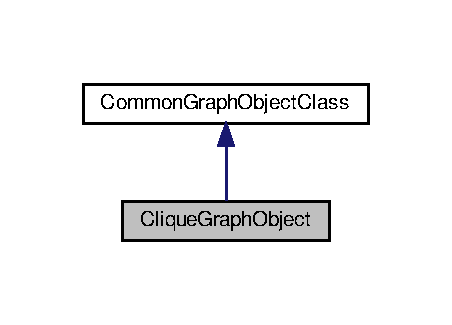
\includegraphics[width=217pt]{classCliqueGraphObject__inherit__graph}
\end{center}
\end{figure}


Collaboration diagram for Clique\+Graph\+Object\+:
\nopagebreak
\begin{figure}[H]
\begin{center}
\leavevmode
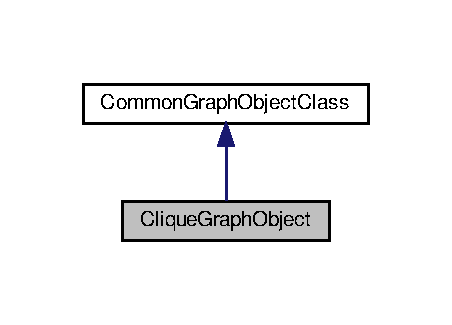
\includegraphics[width=217pt]{classCliqueGraphObject__coll__graph}
\end{center}
\end{figure}
\subsection*{Public Member Functions}
\begin{DoxyCompactItemize}
\item 
\mbox{\Hypertarget{classCliqueGraphObject_a55132ef307105aacf09868e308d6d52f}\label{classCliqueGraphObject_a55132ef307105aacf09868e308d6d52f}} 
{\bfseries Clique\+Graph\+Object} (unsigned long num\+\_\+nodes)
\item 
\mbox{\Hypertarget{classCliqueGraphObject_a415a29f1db0ccf20e75679bf2833d463}\label{classCliqueGraphObject_a415a29f1db0ccf20e75679bf2833d463}} 
void {\bfseries build} ()
\end{DoxyCompactItemize}
\subsection*{Public Attributes}
\begin{DoxyCompactItemize}
\item 
\mbox{\Hypertarget{classCliqueGraphObject_a1939c1fc1a272993642483907549bd71}\label{classCliqueGraphObject_a1939c1fc1a272993642483907549bd71}} 
unsigned long {\bfseries N}
\item 
\mbox{\Hypertarget{classCliqueGraphObject_a4faceb0a6fecb58101d0ab8f7387b465}\label{classCliqueGraphObject_a4faceb0a6fecb58101d0ab8f7387b465}} 
unsigned long {\bfseries E}
\item 
\mbox{\Hypertarget{classCliqueGraphObject_ab1ea07882335176bcc4294ef47d312c7}\label{classCliqueGraphObject_ab1ea07882335176bcc4294ef47d312c7}} 
Graph {\bfseries g}
\item 
\mbox{\Hypertarget{classCliqueGraphObject_ae67ffb085c1b077a7d9a8577ccfbf4b2}\label{classCliqueGraphObject_ae67ffb085c1b077a7d9a8577ccfbf4b2}} 
unsigned long {\bfseries Procs} = num\+\_\+processes(boost\+::graph\+::distributed\+::mpi\+\_\+process\+\_\+group())
\end{DoxyCompactItemize}


The documentation for this class was generated from the following files\+:\begin{DoxyCompactItemize}
\item 
Graph\+Classes/Clique\+Graph.\+h\item 
Graph\+Classes/Clique\+Graph.\+cpp\end{DoxyCompactItemize}

\hypertarget{classCommonGraphObjectClass}{}\section{Common\+Graph\+Object\+Class Class Reference}
\label{classCommonGraphObjectClass}\index{Common\+Graph\+Object\+Class@{Common\+Graph\+Object\+Class}}


Inheritance diagram for Common\+Graph\+Object\+Class\+:
\nopagebreak
\begin{figure}[H]
\begin{center}
\leavevmode
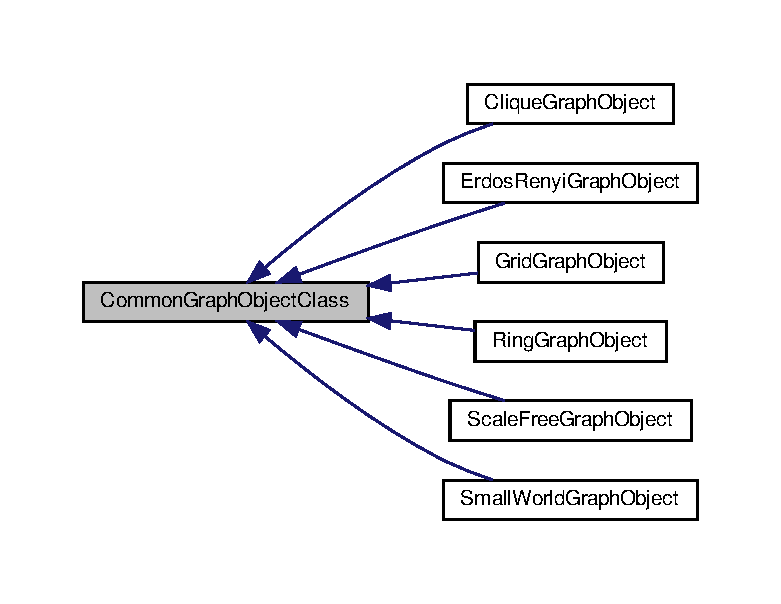
\includegraphics[width=350pt]{classCommonGraphObjectClass__inherit__graph}
\end{center}
\end{figure}
\subsection*{Public Member Functions}
\begin{DoxyCompactItemize}
\item 
\mbox{\Hypertarget{classCommonGraphObjectClass_aa9c64c62cc9660a8c261f660ccca4d68}\label{classCommonGraphObjectClass_aa9c64c62cc9660a8c261f660ccca4d68}} 
void {\bfseries show\+Vertex} (Graph \&g)
\item 
\mbox{\Hypertarget{classCommonGraphObjectClass_a7ba9ff5d091d1e5b29f8b7fcd6215e53}\label{classCommonGraphObjectClass_a7ba9ff5d091d1e5b29f8b7fcd6215e53}} 
void {\bfseries show\+Edges} (Graph \&g)
\item 
\mbox{\Hypertarget{classCommonGraphObjectClass_ac193f6ba2806127a365aa391db9e2fa8}\label{classCommonGraphObjectClass_ac193f6ba2806127a365aa391db9e2fa8}} 
void {\bfseries report\+N\+Procs} (Graph \&g)
\item 
\mbox{\Hypertarget{classCommonGraphObjectClass_a538f35e0b827018171beed35c579d3af}\label{classCommonGraphObjectClass_a538f35e0b827018171beed35c579d3af}} 
void {\bfseries report\+Nodes} (Graph \&g)
\item 
\mbox{\Hypertarget{classCommonGraphObjectClass_a6239be7bef168bc0c13301f50f50b05d}\label{classCommonGraphObjectClass_a6239be7bef168bc0c13301f50f50b05d}} 
void {\bfseries Initialization} (std\+::vector$<$ std\+::pair$<$ double, double $>$$>$ X0\+\_\+W, double J, Graph \&g, unsigned int N)
\end{DoxyCompactItemize}


The documentation for this class was generated from the following files\+:\begin{DoxyCompactItemize}
\item 
Graph\+Classes/General\+Graph.\+h\item 
Graph\+Classes/General\+Graph.\+cpp\end{DoxyCompactItemize}

\hypertarget{structDynamicEdge}{}\section{Dynamic\+Edge Struct Reference}
\label{structDynamicEdge}\index{Dynamic\+Edge@{Dynamic\+Edge}}
\subsection*{Public Member Functions}
\begin{DoxyCompactItemize}
\item 
\mbox{\Hypertarget{structDynamicEdge_ac6924c98f001d82ba565c9fedd2e3c87}\label{structDynamicEdge_ac6924c98f001d82ba565c9fedd2e3c87}} 
{\bfseries Dynamic\+Edge} (double i)
\item 
\mbox{\Hypertarget{structDynamicEdge_a685fb1ed1035f87f7095f64a9746202f}\label{structDynamicEdge_a685fb1ed1035f87f7095f64a9746202f}} 
{\footnotesize template$<$typename Archiver $>$ }\\void {\bfseries serialize} (Archiver \&ar, const unsigned int)
\end{DoxyCompactItemize}
\subsection*{Public Attributes}
\begin{DoxyCompactItemize}
\item 
\mbox{\Hypertarget{structDynamicEdge_a8131459b38901852752f787e42c991aa}\label{structDynamicEdge_a8131459b38901852752f787e42c991aa}} 
double {\bfseries value} = 1
\end{DoxyCompactItemize}


The documentation for this struct was generated from the following file\+:\begin{DoxyCompactItemize}
\item 
Graph\+Classes/General\+Graph.\+h\end{DoxyCompactItemize}

\hypertarget{structDynamicNode}{}\section{Dynamic\+Node Struct Reference}
\label{structDynamicNode}\index{Dynamic\+Node@{Dynamic\+Node}}
\subsection*{Public Member Functions}
\begin{DoxyCompactItemize}
\item 
\mbox{\Hypertarget{structDynamicNode_a96cf410a841d736bb55b410dd8ae41ed}\label{structDynamicNode_a96cf410a841d736bb55b410dd8ae41ed}} 
{\bfseries Dynamic\+Node} (double i)
\item 
\mbox{\Hypertarget{structDynamicNode_a213fbd6be0876b04cb6d24549bf209f5}\label{structDynamicNode_a213fbd6be0876b04cb6d24549bf209f5}} 
{\footnotesize template$<$typename Archiver $>$ }\\void {\bfseries serialize} (Archiver \&ar, const unsigned int)
\end{DoxyCompactItemize}
\subsection*{Public Attributes}
\begin{DoxyCompactItemize}
\item 
\mbox{\Hypertarget{structDynamicNode_afe4e467d9efaf4c2fac54df7a3c561da}\label{structDynamicNode_afe4e467d9efaf4c2fac54df7a3c561da}} 
double {\bfseries value} = 0
\item 
\mbox{\Hypertarget{structDynamicNode_a48f76ef3032dd0c76e618e62a09cb634}\label{structDynamicNode_a48f76ef3032dd0c76e618e62a09cb634}} 
double {\bfseries temporal\+\_\+register} = 0
\item 
\mbox{\Hypertarget{structDynamicNode_a81c008fff53985466c78dfae406413a6}\label{structDynamicNode_a81c008fff53985466c78dfae406413a6}} 
std\+::vector$<$ double $>$ {\bfseries params}
\end{DoxyCompactItemize}


The documentation for this struct was generated from the following file\+:\begin{DoxyCompactItemize}
\item 
Graph\+Classes/General\+Graph.\+h\end{DoxyCompactItemize}

\hypertarget{classErdosRenyiGraphObject}{}\section{Erdos\+Renyi\+Graph\+Object Class Reference}
\label{classErdosRenyiGraphObject}\index{Erdos\+Renyi\+Graph\+Object@{Erdos\+Renyi\+Graph\+Object}}


Inheritance diagram for Erdos\+Renyi\+Graph\+Object\+:
\nopagebreak
\begin{figure}[H]
\begin{center}
\leavevmode
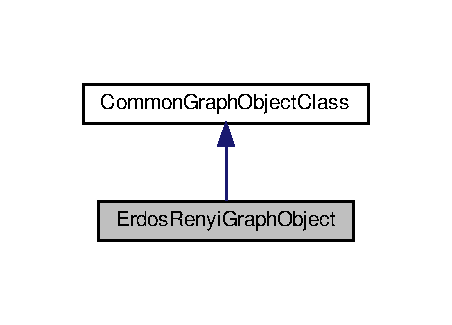
\includegraphics[width=217pt]{classErdosRenyiGraphObject__inherit__graph}
\end{center}
\end{figure}


Collaboration diagram for Erdos\+Renyi\+Graph\+Object\+:
\nopagebreak
\begin{figure}[H]
\begin{center}
\leavevmode
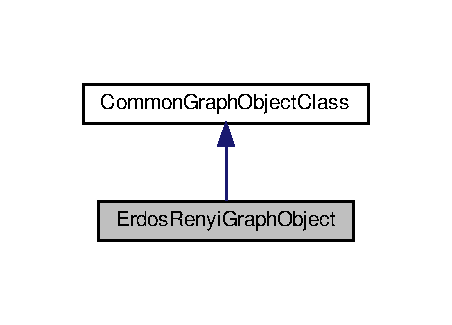
\includegraphics[width=217pt]{classErdosRenyiGraphObject__coll__graph}
\end{center}
\end{figure}
\subsection*{Public Types}
\begin{DoxyCompactItemize}
\item 
\mbox{\Hypertarget{classErdosRenyiGraphObject_a604e71001c96c8b45111302fc00a977a}\label{classErdosRenyiGraphObject_a604e71001c96c8b45111302fc00a977a}} 
typedef boost\+::sorted\+\_\+erdos\+\_\+renyi\+\_\+iterator$<$ boost\+::minstd\+\_\+rand, Graph $>$ {\bfseries E\+R\+Gen}
\end{DoxyCompactItemize}
\subsection*{Public Member Functions}
\begin{DoxyCompactItemize}
\item 
\mbox{\Hypertarget{classErdosRenyiGraphObject_ab0b1e8a1e89891ddf11069dee9343209}\label{classErdosRenyiGraphObject_ab0b1e8a1e89891ddf11069dee9343209}} 
{\bfseries Erdos\+Renyi\+Graph\+Object} (unsigned long num\+\_\+nodes, double probability)
\item 
\mbox{\Hypertarget{classErdosRenyiGraphObject_abc4d4b8856503811bafc314e1a8f8e9e}\label{classErdosRenyiGraphObject_abc4d4b8856503811bafc314e1a8f8e9e}} 
void {\bfseries build} ()
\end{DoxyCompactItemize}
\subsection*{Public Attributes}
\begin{DoxyCompactItemize}
\item 
\mbox{\Hypertarget{classErdosRenyiGraphObject_a1f325e8c05b6b6d18eabc9c5edb9db1c}\label{classErdosRenyiGraphObject_a1f325e8c05b6b6d18eabc9c5edb9db1c}} 
unsigned long {\bfseries N}
\item 
\mbox{\Hypertarget{classErdosRenyiGraphObject_a6eeee359c03d9b94fb9098e386da2010}\label{classErdosRenyiGraphObject_a6eeee359c03d9b94fb9098e386da2010}} 
unsigned long {\bfseries E}
\item 
\mbox{\Hypertarget{classErdosRenyiGraphObject_a4d57ccaf608593ef8b5529c19b65424c}\label{classErdosRenyiGraphObject_a4d57ccaf608593ef8b5529c19b65424c}} 
Graph {\bfseries g}
\item 
\mbox{\Hypertarget{classErdosRenyiGraphObject_a3e074970e0a0e70815b9d9b7a5af5606}\label{classErdosRenyiGraphObject_a3e074970e0a0e70815b9d9b7a5af5606}} 
boost\+::minstd\+\_\+rand {\bfseries gen}
\item 
\mbox{\Hypertarget{classErdosRenyiGraphObject_a3f3449302cf97157245f1502616d6008}\label{classErdosRenyiGraphObject_a3f3449302cf97157245f1502616d6008}} 
double {\bfseries Proba}
\item 
\mbox{\Hypertarget{classErdosRenyiGraphObject_a1e768ea11a266d6cc5b05819e02d1dc2}\label{classErdosRenyiGraphObject_a1e768ea11a266d6cc5b05819e02d1dc2}} 
unsigned long {\bfseries Procs} = num\+\_\+processes(boost\+::graph\+::distributed\+::mpi\+\_\+process\+\_\+group())
\end{DoxyCompactItemize}


The documentation for this class was generated from the following file\+:\begin{DoxyCompactItemize}
\item 
Graph\+Classes/Erdos\+Renyi\+Graph.\+h\end{DoxyCompactItemize}

\hypertarget{classEulerSolver}{}\section{Euler\+Solver$<$ Equation $>$ Class Template Reference}
\label{classEulerSolver}\index{Euler\+Solver$<$ Equation $>$@{Euler\+Solver$<$ Equation $>$}}
\subsection*{Public Member Functions}
\begin{DoxyCompactItemize}
\item 
\mbox{\Hypertarget{classEulerSolver_aa2d39ebf15960d4d6cb6b0b02213e253}\label{classEulerSolver_aa2d39ebf15960d4d6cb6b0b02213e253}} 
void {\bfseries evolve} (double t, double h, double a, std\+::vector$<$ double $>$ \&b, std\+::vector$<$ double $>$ \&c, std\+::vector$<$ double $>$ \&d, Equation \&E, \hyperlink{structFlowSpecs}{Flow\+Specs} \&Specs, std\+::vector$<$ double $>$ \&R\+K1, std\+::vector$<$ double $>$ \&R\+K2, std\+::vector$<$ double $>$ \&R\+K3, std\+::vector$<$ double $>$ \&R\+K4, double \&answer, double $\ast$P)
\item 
\mbox{\Hypertarget{classEulerSolver_acc7ad686da6a0022b6b765f3819ff14f}\label{classEulerSolver_acc7ad686da6a0022b6b765f3819ff14f}} 
void {\bfseries Term1} (double t, double h, double a, std\+::vector$<$ double $>$ \&b, std\+::vector$<$ double $>$ \&c, std\+::vector$<$ double $>$ \&d, Equation \&E, \hyperlink{structFlowSpecs}{Flow\+Specs} \&Specs, std\+::vector$<$ double $>$ \&R\+K1, double $\ast$P)
\item 
\mbox{\Hypertarget{classEulerSolver_a983fba06c599c0a58348c588555b8f28}\label{classEulerSolver_a983fba06c599c0a58348c588555b8f28}} 
void {\bfseries Term2} (double t, double h, double a, std\+::vector$<$ double $>$ \&b, std\+::vector$<$ double $>$ \&c, std\+::vector$<$ double $>$ \&d, Equation \&E, \hyperlink{structFlowSpecs}{Flow\+Specs} \&Specs, std\+::vector$<$ double $>$ \&R\+K1, std\+::vector$<$ double $>$ \&R\+K2, double $\ast$P)
\item 
\mbox{\Hypertarget{classEulerSolver_a2cead92011bfba627c84294652bc50bc}\label{classEulerSolver_a2cead92011bfba627c84294652bc50bc}} 
void {\bfseries Term3} (double t, double h, double a, std\+::vector$<$ double $>$ \&b, std\+::vector$<$ double $>$ \&c, std\+::vector$<$ double $>$ \&d, Equation \&E, \hyperlink{structFlowSpecs}{Flow\+Specs} \&Specs, std\+::vector$<$ double $>$ \&R\+K1, std\+::vector$<$ double $>$ \&R\+K2, std\+::vector$<$ double $>$ \&R\+K3, double $\ast$P)
\item 
\mbox{\Hypertarget{classEulerSolver_a5d0977e97c90e60e407f611c76459082}\label{classEulerSolver_a5d0977e97c90e60e407f611c76459082}} 
void {\bfseries Term4} (double t, double h, double a, std\+::vector$<$ double $>$ \&b, std\+::vector$<$ double $>$ \&c, std\+::vector$<$ double $>$ \&d, Equation \&E, \hyperlink{structFlowSpecs}{Flow\+Specs} \&Specs, std\+::vector$<$ double $>$ \&R\+K1, std\+::vector$<$ double $>$ \&R\+K2, std\+::vector$<$ double $>$ \&R\+K3, std\+::vector$<$ double $>$ \&R\+K4, double $\ast$P)
\end{DoxyCompactItemize}


The documentation for this class was generated from the following file\+:\begin{DoxyCompactItemize}
\item 
Solvers/Euler\+Solver.\+h\end{DoxyCompactItemize}

\hypertarget{classFieldRequestObject}{}\section{Field\+Request\+Object$<$ field $>$ Class Template Reference}
\label{classFieldRequestObject}\index{Field\+Request\+Object$<$ field $>$@{Field\+Request\+Object$<$ field $>$}}
\subsection*{Public Types}
\begin{DoxyCompactItemize}
\item 
\mbox{\Hypertarget{classFieldRequestObject_a6ad4716d361d230f2c5d595a02834676}\label{classFieldRequestObject_a6ad4716d361d230f2c5d595a02834676}} 
typedef std\+::conditional$<$(field $>$=0), int, double $>$\+::type {\bfseries buffer\+\_\+type}
\item 
\mbox{\Hypertarget{classFieldRequestObject_a639b3bfa2074c23a6d9931a7a2ddbc5f}\label{classFieldRequestObject_a639b3bfa2074c23a6d9931a7a2ddbc5f}} 
typedef std\+::conditional$<$(field $>$=-\/2), double, double $>$\+::type {\bfseries answer\+\_\+type}
\end{DoxyCompactItemize}
\subsection*{Public Member Functions}
\begin{DoxyCompactItemize}
\item 
\mbox{\Hypertarget{classFieldRequestObject_a8522242a8ba5892063c3e74350c8ada1}\label{classFieldRequestObject_a8522242a8ba5892063c3e74350c8ada1}} 
void {\bfseries build\+Send\+Tag} (int $\ast$data)
\item 
\mbox{\Hypertarget{classFieldRequestObject_a62b6f677a3c63324d17983c3db9cd45e}\label{classFieldRequestObject_a62b6f677a3c63324d17983c3db9cd45e}} 
void {\bfseries build\+Send\+Tag} (double $\ast$data)
\item 
\mbox{\Hypertarget{classFieldRequestObject_a887b9bd282d07f20833d38116c162f03}\label{classFieldRequestObject_a887b9bd282d07f20833d38116c162f03}} 
void {\bfseries build\+Recv\+Tag} (int $\ast$data)
\item 
\mbox{\Hypertarget{classFieldRequestObject_ae13ca2b4dc1426f300a4b9bc463d7a33}\label{classFieldRequestObject_ae13ca2b4dc1426f300a4b9bc463d7a33}} 
void {\bfseries build\+Recv\+Tag} (double $\ast$data)
\item 
\mbox{\Hypertarget{classFieldRequestObject_acb9923d7cdfe59d99f0172e29387a0ed}\label{classFieldRequestObject_acb9923d7cdfe59d99f0172e29387a0ed}} 
void {\bfseries build\+Recv\+Tag} ()
\item 
\mbox{\Hypertarget{classFieldRequestObject_afda006103a3b1c5766c7b87f72193097}\label{classFieldRequestObject_afda006103a3b1c5766c7b87f72193097}} 
void {\bfseries compute\+Answer} (Reference\+Container \&R\+EF, int $\ast$buffer, double $\ast$answer, M\+P\+I\+\_\+\+Status \&S, int M\+Y\+P\+R\+OC)
\item 
\mbox{\Hypertarget{classFieldRequestObject_a5767264fc2688f83215023e3b7131f91}\label{classFieldRequestObject_a5767264fc2688f83215023e3b7131f91}} 
void {\bfseries compute\+Ready} (Reference\+Container \&R\+EF, int $\ast$buffer, bool \&is\+Ready)
\item 
\mbox{\Hypertarget{classFieldRequestObject_a1df3f4397288d977a288514dd88d50d5}\label{classFieldRequestObject_a1df3f4397288d977a288514dd88d50d5}} 
void {\bfseries compute\+Ready} (Reference\+Container \&R\+EF, double $\ast$buffer, bool \&is\+Ready)
\item 
\mbox{\Hypertarget{classFieldRequestObject_a11965c293f75bf51635a69a3588739c2}\label{classFieldRequestObject_a11965c293f75bf51635a69a3588739c2}} 
void {\bfseries compute\+Answer} (Reference\+Container \&R\+EF, double $\ast$buffer, double $\ast$answer, M\+P\+I\+\_\+\+Status \&S, int M\+Y\+P\+R\+OC)
\end{DoxyCompactItemize}
\subsection*{Public Attributes}
\begin{DoxyCompactItemize}
\item 
\mbox{\Hypertarget{classFieldRequestObject_a2ad6c3d99c94c58a9420643d3e0b653d}\label{classFieldRequestObject_a2ad6c3d99c94c58a9420643d3e0b653d}} 
int {\bfseries recv\+Length} = -\/1
\item 
\mbox{\Hypertarget{classFieldRequestObject_a43659bae4495b2924f15e31c05bbe4b7}\label{classFieldRequestObject_a43659bae4495b2924f15e31c05bbe4b7}} 
int {\bfseries send\+Length} = -\/1
\item 
\mbox{\Hypertarget{classFieldRequestObject_a403abbe6c557055936bc46d7587f78ed}\label{classFieldRequestObject_a403abbe6c557055936bc46d7587f78ed}} 
int {\bfseries recv\+Tag} = -\/1
\item 
\mbox{\Hypertarget{classFieldRequestObject_ad7e1aa4729c8b9ac854975e90cbb5cfb}\label{classFieldRequestObject_ad7e1aa4729c8b9ac854975e90cbb5cfb}} 
int {\bfseries send\+Tag} = -\/1
\item 
\mbox{\Hypertarget{classFieldRequestObject_a6f900d722138b5826988f49375ff4689}\label{classFieldRequestObject_a6f900d722138b5826988f49375ff4689}} 
bool {\bfseries recv\+Int} = true
\item 
\mbox{\Hypertarget{classFieldRequestObject_aeed51f8a97bf6175052c899525482ad9}\label{classFieldRequestObject_aeed51f8a97bf6175052c899525482ad9}} 
bool {\bfseries send\+Double} = true
\end{DoxyCompactItemize}


The documentation for this class was generated from the following file\+:\begin{DoxyCompactItemize}
\item 
Communication/Communication\+Functions.\+h\end{DoxyCompactItemize}

\hypertarget{structFlowSpecs}{}\section{Flow\+Specs Struct Reference}
\label{structFlowSpecs}\index{Flow\+Specs@{Flow\+Specs}}
\subsection*{Public Member Functions}
\begin{DoxyCompactItemize}
\item 
\mbox{\Hypertarget{structFlowSpecs_a4afc47d62dc346f382b3bcb26440642f}\label{structFlowSpecs_a4afc47d62dc346f382b3bcb26440642f}} 
{\bfseries Flow\+Specs} (std\+::vector$<$ double $>$ T1, std\+::vector$<$ double $>$ T2, std\+::vector$<$ double $>$ T3, std\+::vector$<$ double $>$ T4, int N)
\end{DoxyCompactItemize}
\subsection*{Public Attributes}
\begin{DoxyCompactItemize}
\item 
\mbox{\Hypertarget{structFlowSpecs_a5a27437ab644c00f64f92071a2f76856}\label{structFlowSpecs_a5a27437ab644c00f64f92071a2f76856}} 
std\+::vector$<$ double $>$ {\bfseries T1}
\item 
\mbox{\Hypertarget{structFlowSpecs_a8fd50e0322b69a2122ce3928fcc3c0aa}\label{structFlowSpecs_a8fd50e0322b69a2122ce3928fcc3c0aa}} 
std\+::vector$<$ double $>$ {\bfseries T2}
\item 
\mbox{\Hypertarget{structFlowSpecs_a93d29e97f0c611a8dcfd929de06606d3}\label{structFlowSpecs_a93d29e97f0c611a8dcfd929de06606d3}} 
std\+::vector$<$ double $>$ {\bfseries T3}
\item 
\mbox{\Hypertarget{structFlowSpecs_a1aa0d8d815aec2e1a754d518bc3ffa5e}\label{structFlowSpecs_a1aa0d8d815aec2e1a754d518bc3ffa5e}} 
std\+::vector$<$ double $>$ {\bfseries T4}
\item 
\mbox{\Hypertarget{structFlowSpecs_ac4ffae186508f9eba2b027f5bb2e9617}\label{structFlowSpecs_ac4ffae186508f9eba2b027f5bb2e9617}} 
int {\bfseries N}
\item 
\mbox{\Hypertarget{structFlowSpecs_a2eea620572185c537a33ac2e4e63d57e}\label{structFlowSpecs_a2eea620572185c537a33ac2e4e63d57e}} 
int {\bfseries j1}
\item 
\mbox{\Hypertarget{structFlowSpecs_a1af5426798d95ccb302e7304c4b9cdbe}\label{structFlowSpecs_a1af5426798d95ccb302e7304c4b9cdbe}} 
int {\bfseries j2}
\item 
\mbox{\Hypertarget{structFlowSpecs_a7d4ddd5f7fb9974282eb49d12a9e7388}\label{structFlowSpecs_a7d4ddd5f7fb9974282eb49d12a9e7388}} 
int {\bfseries j3}
\item 
\mbox{\Hypertarget{structFlowSpecs_ab41aa036402a0684acfd20dc340e8481}\label{structFlowSpecs_ab41aa036402a0684acfd20dc340e8481}} 
int {\bfseries j4}
\item 
\mbox{\Hypertarget{structFlowSpecs_a4b30677d87454530a327bce3ec97d2ca}\label{structFlowSpecs_a4b30677d87454530a327bce3ec97d2ca}} 
double {\bfseries result}
\end{DoxyCompactItemize}


The documentation for this struct was generated from the following file\+:\begin{DoxyCompactItemize}
\item 
Differential\+Equations/General\+Differential\+Equation.\+h\end{DoxyCompactItemize}

\hypertarget{classGeneralDifferentialEquation}{}\section{General\+Differential\+Equation Class Reference}
\label{classGeneralDifferentialEquation}\index{General\+Differential\+Equation@{General\+Differential\+Equation}}


Inheritance diagram for General\+Differential\+Equation\+:
\nopagebreak
\begin{figure}[H]
\begin{center}
\leavevmode
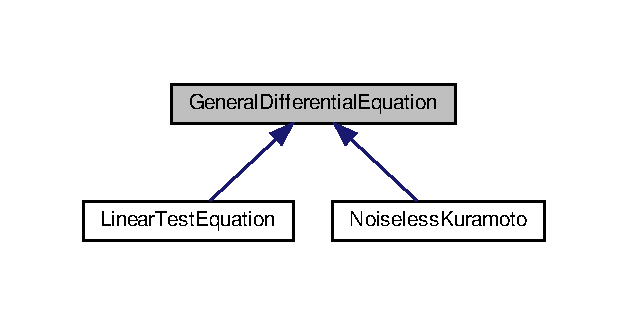
\includegraphics[width=302pt]{classGeneralDifferentialEquation__inherit__graph}
\end{center}
\end{figure}


Collaboration diagram for General\+Differential\+Equation\+:
\nopagebreak
\begin{figure}[H]
\begin{center}
\leavevmode
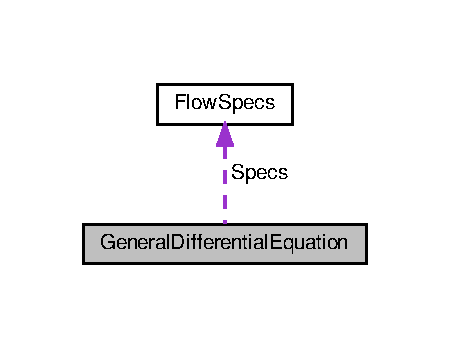
\includegraphics[width=216pt]{classGeneralDifferentialEquation__coll__graph}
\end{center}
\end{figure}
\subsection*{Public Member Functions}
\begin{DoxyCompactItemize}
\item 
\mbox{\Hypertarget{classGeneralDifferentialEquation_a4cbcdc8a02814d8a7fd4a0c3396f2cbd}\label{classGeneralDifferentialEquation_a4cbcdc8a02814d8a7fd4a0c3396f2cbd}} 
{\bfseries General\+Differential\+Equation} (int type)
\item 
\mbox{\Hypertarget{classGeneralDifferentialEquation_a2822b2cb9303f156f235babd48fbf2a7}\label{classGeneralDifferentialEquation_a2822b2cb9303f156f235babd48fbf2a7}} 
void {\bfseries Update\+Flow\+Specs} (std\+::vector$<$ double $>$ \&T1, std\+::vector$<$ double $>$ \&T2, std\+::vector$<$ double $>$ \&T3, std\+::vector$<$ double $>$ \&T4, int N)
\item 
\mbox{\Hypertarget{classGeneralDifferentialEquation_ad0cc54c8051369a2fa05ae9b1679c89c}\label{classGeneralDifferentialEquation_ad0cc54c8051369a2fa05ae9b1679c89c}} 
void {\bfseries Reset} ()
\item 
\mbox{\Hypertarget{classGeneralDifferentialEquation_aaaeffd92dc367daa473dfb0a12e6c3e6}\label{classGeneralDifferentialEquation_aaaeffd92dc367daa473dfb0a12e6c3e6}} 
void {\bfseries Build\+For\+Solver} ()
\end{DoxyCompactItemize}
\subsection*{Public Attributes}
\begin{DoxyCompactItemize}
\item 
\mbox{\Hypertarget{classGeneralDifferentialEquation_a5e74b72eaad71cfaef6cd67881cb0033}\label{classGeneralDifferentialEquation_a5e74b72eaad71cfaef6cd67881cb0033}} 
int {\bfseries type}
\item 
\mbox{\Hypertarget{classGeneralDifferentialEquation_a4af7ed36584cc27ba75848aaf7383fe3}\label{classGeneralDifferentialEquation_a4af7ed36584cc27ba75848aaf7383fe3}} 
bool {\bfseries Requires\+Building} = false
\item 
\mbox{\Hypertarget{classGeneralDifferentialEquation_aea4ad56284abaa02afde25027e35116d}\label{classGeneralDifferentialEquation_aea4ad56284abaa02afde25027e35116d}} 
\hyperlink{structFlowSpecs}{Flow\+Specs} {\bfseries Specs}
\end{DoxyCompactItemize}


The documentation for this class was generated from the following files\+:\begin{DoxyCompactItemize}
\item 
Differential\+Equations/General\+Differential\+Equation.\+h\item 
Differential\+Equations/General\+Differential\+Equation.\+cpp\end{DoxyCompactItemize}

\hypertarget{classGeneralSolver}{}\section{General\+Solver$<$ D\+I\+F\+F\+EQ, S\+O\+L\+V\+ER $>$ Class Template Reference}
\label{classGeneralSolver}\index{General\+Solver$<$ D\+I\+F\+F\+E\+Q, S\+O\+L\+V\+E\+R $>$@{General\+Solver$<$ D\+I\+F\+F\+E\+Q, S\+O\+L\+V\+E\+R $>$}}


Collaboration diagram for General\+Solver$<$ D\+I\+F\+F\+EQ, S\+O\+L\+V\+ER $>$\+:
\nopagebreak
\begin{figure}[H]
\begin{center}
\leavevmode
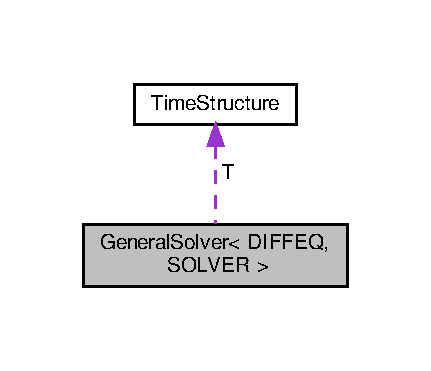
\includegraphics[width=207pt]{classGeneralSolver__coll__graph}
\end{center}
\end{figure}
\subsection*{Public Member Functions}
\begin{DoxyCompactItemize}
\item 
\mbox{\Hypertarget{classGeneralSolver_ab558a72e287752a64449810029ef036f}\label{classGeneralSolver_ab558a72e287752a64449810029ef036f}} 
{\bfseries General\+Solver} (std\+::string valtype)
\item 
\mbox{\Hypertarget{classGeneralSolver_a5a8d5e0b856b0fb7fb7a05fd6da84fcb}\label{classGeneralSolver_a5a8d5e0b856b0fb7fb7a05fd6da84fcb}} 
{\bfseries General\+Solver} (std\+::string valtype, int d)
\item 
\mbox{\Hypertarget{classGeneralSolver_a79d402c597f2e84337d89036eba4ef9b}\label{classGeneralSolver_a79d402c597f2e84337d89036eba4ef9b}} 
{\bfseries General\+Solver} (std\+::string valtype, int d, double $\ast$params)
\item 
\mbox{\Hypertarget{classGeneralSolver_af26d2bd217b8b2303d5c41d60376588c}\label{classGeneralSolver_af26d2bd217b8b2303d5c41d60376588c}} 
void {\bfseries Post\+Template\+Processing} ()
\item 
\mbox{\Hypertarget{classGeneralSolver_a35bc9d64300be88f4a64d426016018c4}\label{classGeneralSolver_a35bc9d64300be88f4a64d426016018c4}} 
void {\bfseries evolve} (double a, std\+::vector$<$ double $>$ \&b, std\+::vector$<$ double $>$ \&c, std\+::vector$<$ double $>$ \&d, std\+::vector$<$ double $>$ \&R\+K1, std\+::vector$<$ double $>$ \&R\+K2, std\+::vector$<$ double $>$ \&R\+K3, std\+::vector$<$ double $>$ \&R\+K4, double \&answer)
\item 
\mbox{\Hypertarget{classGeneralSolver_a6d8ecaeb7aa8833616f94e526e9ecf75}\label{classGeneralSolver_a6d8ecaeb7aa8833616f94e526e9ecf75}} 
void {\bfseries Term1} (double a, std\+::vector$<$ double $>$ \&b, std\+::vector$<$ double $>$ \&c, std\+::vector$<$ double $>$ \&d, std\+::vector$<$ double $>$ \&R\+K1)
\item 
\mbox{\Hypertarget{classGeneralSolver_aff0944c9a83904ca7f06b49bd4a30e62}\label{classGeneralSolver_aff0944c9a83904ca7f06b49bd4a30e62}} 
void {\bfseries Term2} (double a, std\+::vector$<$ double $>$ \&b, std\+::vector$<$ double $>$ \&c, std\+::vector$<$ double $>$ \&d, std\+::vector$<$ double $>$ \&R\+K1, std\+::vector$<$ double $>$ \&R\+K2)
\item 
\mbox{\Hypertarget{classGeneralSolver_a36e8b1a601b8eaa6e9fdb9db33d1c82e}\label{classGeneralSolver_a36e8b1a601b8eaa6e9fdb9db33d1c82e}} 
void {\bfseries Term3} (double a, std\+::vector$<$ double $>$ \&b, std\+::vector$<$ double $>$ \&c, std\+::vector$<$ double $>$ \&d, std\+::vector$<$ double $>$ \&R\+K1, std\+::vector$<$ double $>$ \&R\+K2, std\+::vector$<$ double $>$ \&R\+K3)
\item 
\mbox{\Hypertarget{classGeneralSolver_a656257a26a068283f5e296a0c800baf6}\label{classGeneralSolver_a656257a26a068283f5e296a0c800baf6}} 
void {\bfseries Term4} (double a, std\+::vector$<$ double $>$ \&b, std\+::vector$<$ double $>$ \&c, std\+::vector$<$ double $>$ \&d, std\+::vector$<$ double $>$ \&R\+K1, std\+::vector$<$ double $>$ \&R\+K2, std\+::vector$<$ double $>$ \&R\+K3, std\+::vector$<$ double $>$ \&R\+K4)
\item 
\mbox{\Hypertarget{classGeneralSolver_a37505b19e23e7949e5ec1c95ac556e11}\label{classGeneralSolver_a37505b19e23e7949e5ec1c95ac556e11}} 
void {\bfseries Set\+Step} (double h)
\item 
\mbox{\Hypertarget{classGeneralSolver_a29e088c061743d092a681666599bcfa4}\label{classGeneralSolver_a29e088c061743d092a681666599bcfa4}} 
void {\bfseries Set\+T0} (double t0)
\item 
\mbox{\Hypertarget{classGeneralSolver_a20243a636c94dbdd8bf56873497721f7}\label{classGeneralSolver_a20243a636c94dbdd8bf56873497721f7}} 
void {\bfseries Evolve\+Time} ()
\end{DoxyCompactItemize}
\subsection*{Public Attributes}
\begin{DoxyCompactItemize}
\item 
\mbox{\Hypertarget{classGeneralSolver_aab8c1ef25686ffb53c043e1c1ff098d2}\label{classGeneralSolver_aab8c1ef25686ffb53c043e1c1ff098d2}} 
double {\bfseries Params} \mbox{[}4\mbox{]}
\item 
\mbox{\Hypertarget{classGeneralSolver_ab04759cf4ed2570d988446cfb121c0cc}\label{classGeneralSolver_ab04759cf4ed2570d988446cfb121c0cc}} 
int {\bfseries deg}
\item 
\mbox{\Hypertarget{classGeneralSolver_a44930211006db48661bf9bbef9722ea1}\label{classGeneralSolver_a44930211006db48661bf9bbef9722ea1}} 
std\+::string {\bfseries type}
\item 
\mbox{\Hypertarget{classGeneralSolver_a4adb47207dde1bf87b13c8c04cbbb89f}\label{classGeneralSolver_a4adb47207dde1bf87b13c8c04cbbb89f}} 
bool {\bfseries requires\+\_\+communication} = false
\item 
\mbox{\Hypertarget{classGeneralSolver_a2585069188cd1b9abdf7e66bb029481c}\label{classGeneralSolver_a2585069188cd1b9abdf7e66bb029481c}} 
D\+I\+F\+F\+EQ {\bfseries Differential\+Equation}
\item 
\mbox{\Hypertarget{classGeneralSolver_a56c223b1e7d8679d97bf7f153f09bd07}\label{classGeneralSolver_a56c223b1e7d8679d97bf7f153f09bd07}} 
S\+O\+L\+V\+ER {\bfseries Solver}
\item 
\mbox{\Hypertarget{classGeneralSolver_a6bedad6e0a204022c10363aa8f0bb302}\label{classGeneralSolver_a6bedad6e0a204022c10363aa8f0bb302}} 
\hyperlink{structTimeStructure}{Time\+Structure} {\bfseries T}
\end{DoxyCompactItemize}


The documentation for this class was generated from the following file\+:\begin{DoxyCompactItemize}
\item 
Solvers/General\+Solver.\+h\end{DoxyCompactItemize}

\hypertarget{classGridGraphObject}{}\section{Grid\+Graph\+Object Class Reference}
\label{classGridGraphObject}\index{Grid\+Graph\+Object@{Grid\+Graph\+Object}}


Inheritance diagram for Grid\+Graph\+Object\+:
\nopagebreak
\begin{figure}[H]
\begin{center}
\leavevmode
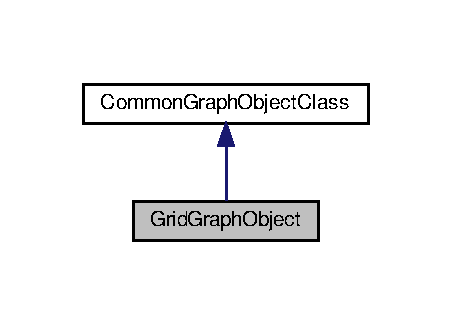
\includegraphics[width=217pt]{classGridGraphObject__inherit__graph}
\end{center}
\end{figure}


Collaboration diagram for Grid\+Graph\+Object\+:
\nopagebreak
\begin{figure}[H]
\begin{center}
\leavevmode
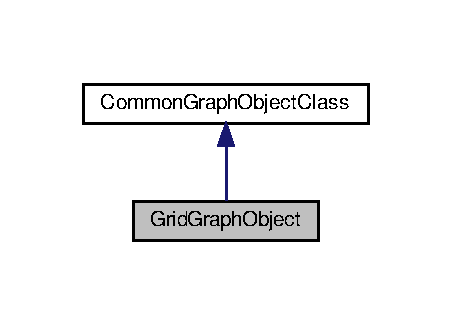
\includegraphics[width=217pt]{classGridGraphObject__coll__graph}
\end{center}
\end{figure}
\subsection*{Public Member Functions}
\begin{DoxyCompactItemize}
\item 
\mbox{\Hypertarget{classGridGraphObject_a981b16c28de44a8fd235e2b0101bdf91}\label{classGridGraphObject_a981b16c28de44a8fd235e2b0101bdf91}} 
{\bfseries Grid\+Graph\+Object} (unsigned long num\+\_\+nodes)
\item 
\mbox{\Hypertarget{classGridGraphObject_ae1ae8c63313364270b36dd074e9dc243}\label{classGridGraphObject_ae1ae8c63313364270b36dd074e9dc243}} 
void {\bfseries build} ()
\end{DoxyCompactItemize}
\subsection*{Public Attributes}
\begin{DoxyCompactItemize}
\item 
\mbox{\Hypertarget{classGridGraphObject_a3cea5ec4a465d4316d40779980fe306b}\label{classGridGraphObject_a3cea5ec4a465d4316d40779980fe306b}} 
unsigned long {\bfseries N}
\item 
\mbox{\Hypertarget{classGridGraphObject_adfe178e009545f42ef05a13322431f09}\label{classGridGraphObject_adfe178e009545f42ef05a13322431f09}} 
unsigned long {\bfseries E}
\item 
\mbox{\Hypertarget{classGridGraphObject_a5781cceddb234c716fbbfa88c5b4228f}\label{classGridGraphObject_a5781cceddb234c716fbbfa88c5b4228f}} 
Graph {\bfseries g}
\item 
\mbox{\Hypertarget{classGridGraphObject_a4d72f7ab2ffd20ea529d0013cc6b2394}\label{classGridGraphObject_a4d72f7ab2ffd20ea529d0013cc6b2394}} 
unsigned long {\bfseries Procs} = num\+\_\+processes(boost\+::graph\+::distributed\+::mpi\+\_\+process\+\_\+group())
\end{DoxyCompactItemize}


The documentation for this class was generated from the following files\+:\begin{DoxyCompactItemize}
\item 
Graph\+Classes/Grid\+Graph.\+h\item 
Graph\+Classes/Grid\+Graph.\+cpp\end{DoxyCompactItemize}

\hypertarget{classLinearTestEquation}{}\section{Linear\+Test\+Equation Class Reference}
\label{classLinearTestEquation}\index{Linear\+Test\+Equation@{Linear\+Test\+Equation}}


Inheritance diagram for Linear\+Test\+Equation\+:
\nopagebreak
\begin{figure}[H]
\begin{center}
\leavevmode
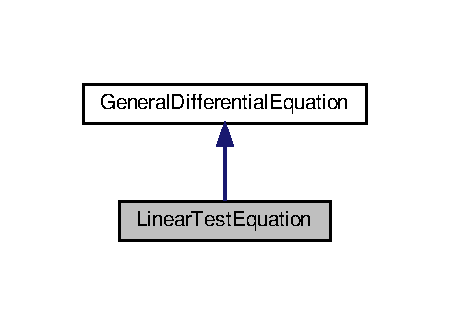
\includegraphics[width=216pt]{classLinearTestEquation__inherit__graph}
\end{center}
\end{figure}


Collaboration diagram for Linear\+Test\+Equation\+:
\nopagebreak
\begin{figure}[H]
\begin{center}
\leavevmode
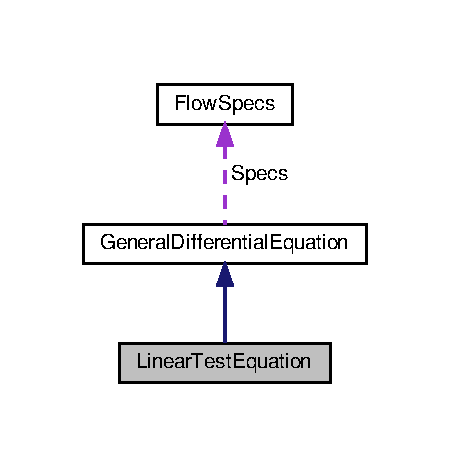
\includegraphics[width=216pt]{classLinearTestEquation__coll__graph}
\end{center}
\end{figure}
\subsection*{Public Member Functions}
\begin{DoxyCompactItemize}
\item 
\mbox{\Hypertarget{classLinearTestEquation_aa7ab524660cc97cbb53fdb78b32dfb9c}\label{classLinearTestEquation_aa7ab524660cc97cbb53fdb78b32dfb9c}} 
bool {\bfseries requires\+Com} (int d)
\item 
\mbox{\Hypertarget{classLinearTestEquation_ac7be044049da8490289be20fde0ffdb5}\label{classLinearTestEquation_ac7be044049da8490289be20fde0ffdb5}} 
void {\bfseries Field} (double t, double a, std\+::vector$<$ double $>$ \&b, std\+::vector$<$ double $>$ \&c, std\+::vector$<$ double $>$ \&d)
\item 
\mbox{\Hypertarget{classLinearTestEquation_ad9ebdc71f9376029b08de9630b8720ef}\label{classLinearTestEquation_ad9ebdc71f9376029b08de9630b8720ef}} 
void {\bfseries d1\+Field} (double t, double a, std\+::vector$<$ double $>$ \&b, std\+::vector$<$ double $>$ \&c, std\+::vector$<$ double $>$ \&d)
\item 
\mbox{\Hypertarget{classLinearTestEquation_aeab6902175fda50de3b4a02921f095ea}\label{classLinearTestEquation_aeab6902175fda50de3b4a02921f095ea}} 
void {\bfseries d2\+Field} (double t, double a, std\+::vector$<$ double $>$ \&b, std\+::vector$<$ double $>$ \&c, std\+::vector$<$ double $>$ \&d)
\item 
\mbox{\Hypertarget{classLinearTestEquation_a9ff6bf55ead037c7fe29fbcc81d0fbf2}\label{classLinearTestEquation_a9ff6bf55ead037c7fe29fbcc81d0fbf2}} 
void {\bfseries d3\+Field} (double t, double a, std\+::vector$<$ double $>$ \&b, std\+::vector$<$ double $>$ \&c, std\+::vector$<$ double $>$ \&d)
\end{DoxyCompactItemize}
\subsection*{Additional Inherited Members}


The documentation for this class was generated from the following files\+:\begin{DoxyCompactItemize}
\item 
Differential\+Equations/Linear\+Test\+Equation.\+h\item 
Differential\+Equations/Linear\+Test\+Equation.\+cpp\end{DoxyCompactItemize}

\hypertarget{classNoiselessKuramoto}{}\section{Noiseless\+Kuramoto Class Reference}
\label{classNoiselessKuramoto}\index{Noiseless\+Kuramoto@{Noiseless\+Kuramoto}}


Inheritance diagram for Noiseless\+Kuramoto\+:
\nopagebreak
\begin{figure}[H]
\begin{center}
\leavevmode
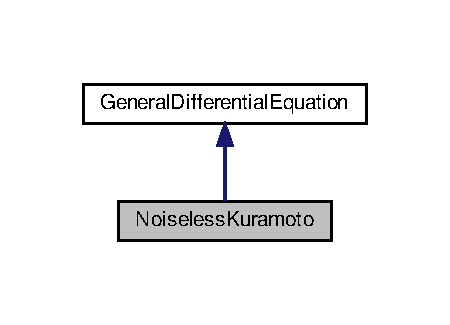
\includegraphics[width=216pt]{classNoiselessKuramoto__inherit__graph}
\end{center}
\end{figure}


Collaboration diagram for Noiseless\+Kuramoto\+:
\nopagebreak
\begin{figure}[H]
\begin{center}
\leavevmode
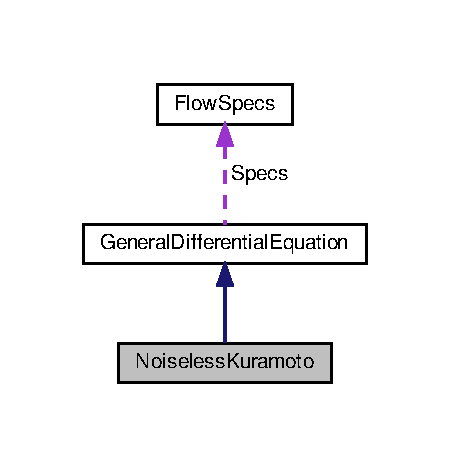
\includegraphics[width=216pt]{classNoiselessKuramoto__coll__graph}
\end{center}
\end{figure}
\subsection*{Public Member Functions}
\begin{DoxyCompactItemize}
\item 
\mbox{\Hypertarget{classNoiselessKuramoto_a895541b3102a4a4326b31b6959d9557c}\label{classNoiselessKuramoto_a895541b3102a4a4326b31b6959d9557c}} 
bool {\bfseries requires\+Com} (int d)
\item 
\mbox{\Hypertarget{classNoiselessKuramoto_ab84a5e300d32b083f66c1cc30ae8ce85}\label{classNoiselessKuramoto_ab84a5e300d32b083f66c1cc30ae8ce85}} 
void {\bfseries Field} (double t, double a, std\+::vector$<$ double $>$ \&b, std\+::vector$<$ double $>$ \&c, std\+::vector$<$ double $>$ \&d)
\item 
\mbox{\Hypertarget{classNoiselessKuramoto_ac53fc879e5b203dac98116a35075472b}\label{classNoiselessKuramoto_ac53fc879e5b203dac98116a35075472b}} 
void {\bfseries d1\+Field} (double t, double a, std\+::vector$<$ double $>$ \&b, std\+::vector$<$ double $>$ \&c, std\+::vector$<$ double $>$ \&d)
\item 
\mbox{\Hypertarget{classNoiselessKuramoto_a530a81415bfd4b425d03036c568a75ff}\label{classNoiselessKuramoto_a530a81415bfd4b425d03036c568a75ff}} 
void {\bfseries d2\+Field} (double t, double a, std\+::vector$<$ double $>$ \&b, std\+::vector$<$ double $>$ \&c, std\+::vector$<$ double $>$ \&d)
\item 
\mbox{\Hypertarget{classNoiselessKuramoto_a6bec0fd694070e867d3956721d235471}\label{classNoiselessKuramoto_a6bec0fd694070e867d3956721d235471}} 
void {\bfseries d3\+Field} (double t, double a, std\+::vector$<$ double $>$ \&b, std\+::vector$<$ double $>$ \&c, std\+::vector$<$ double $>$ \&d)
\end{DoxyCompactItemize}
\subsection*{Additional Inherited Members}


The documentation for this class was generated from the following files\+:\begin{DoxyCompactItemize}
\item 
Differential\+Equations/Noiseless\+Kuramoto.\+h\item 
Differential\+Equations/Noiseless\+Kuramoto.\+cpp\end{DoxyCompactItemize}

\hypertarget{classRequestObject}{}\section{Request\+Object$<$ Specific\+Request\+Object $>$ Class Template Reference}
\label{classRequestObject}\index{Request\+Object$<$ Specific\+Request\+Object $>$@{Request\+Object$<$ Specific\+Request\+Object $>$}}


Inheritance diagram for Request\+Object$<$ Specific\+Request\+Object $>$\+:
\nopagebreak
\begin{figure}[H]
\begin{center}
\leavevmode
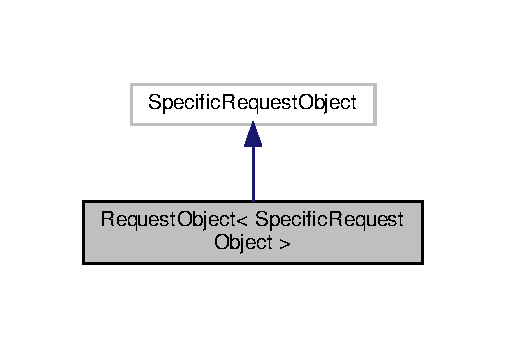
\includegraphics[width=243pt]{classRequestObject__inherit__graph}
\end{center}
\end{figure}


Collaboration diagram for Request\+Object$<$ Specific\+Request\+Object $>$\+:
\nopagebreak
\begin{figure}[H]
\begin{center}
\leavevmode
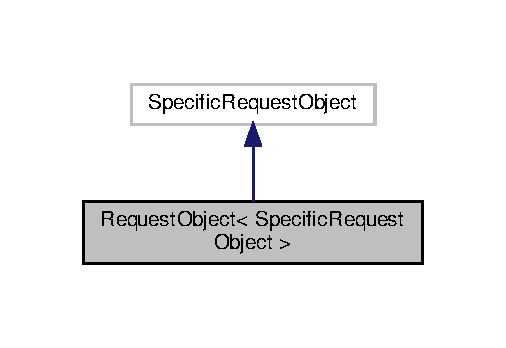
\includegraphics[width=243pt]{classRequestObject__coll__graph}
\end{center}
\end{figure}
\subsection*{Public Member Functions}
\begin{DoxyCompactItemize}
\item 
\mbox{\Hypertarget{classRequestObject_a44075701922d4926e899519df2ce5aed}\label{classRequestObject_a44075701922d4926e899519df2ce5aed}} 
{\bfseries Request\+Object} (int type)
\end{DoxyCompactItemize}


The documentation for this class was generated from the following file\+:\begin{DoxyCompactItemize}
\item 
Communication/Communication\+Functions.\+h\end{DoxyCompactItemize}

\hypertarget{classRingGraphObject}{}\section{Ring\+Graph\+Object Class Reference}
\label{classRingGraphObject}\index{Ring\+Graph\+Object@{Ring\+Graph\+Object}}


Inheritance diagram for Ring\+Graph\+Object\+:
\nopagebreak
\begin{figure}[H]
\begin{center}
\leavevmode
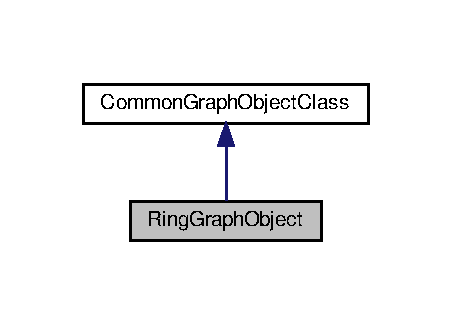
\includegraphics[width=217pt]{classRingGraphObject__inherit__graph}
\end{center}
\end{figure}


Collaboration diagram for Ring\+Graph\+Object\+:
\nopagebreak
\begin{figure}[H]
\begin{center}
\leavevmode
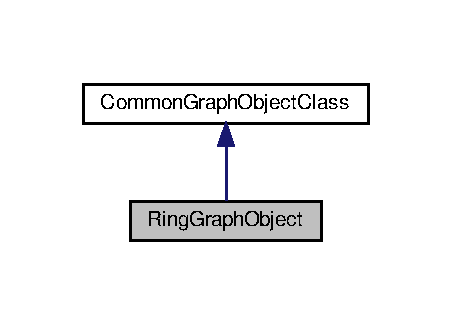
\includegraphics[width=217pt]{classRingGraphObject__coll__graph}
\end{center}
\end{figure}
\subsection*{Public Member Functions}
\begin{DoxyCompactItemize}
\item 
\mbox{\Hypertarget{classRingGraphObject_aa9444a05e454bc4a21564be5ad1b61bf}\label{classRingGraphObject_aa9444a05e454bc4a21564be5ad1b61bf}} 
{\bfseries Ring\+Graph\+Object} (unsigned long num\+\_\+nodes)
\item 
\mbox{\Hypertarget{classRingGraphObject_a9416e0dbcb70a77b9ef58beec72a053e}\label{classRingGraphObject_a9416e0dbcb70a77b9ef58beec72a053e}} 
void {\bfseries build} ()
\end{DoxyCompactItemize}
\subsection*{Public Attributes}
\begin{DoxyCompactItemize}
\item 
\mbox{\Hypertarget{classRingGraphObject_a2e39cfc91f3ddaa28d3cdaa74d5bf8f1}\label{classRingGraphObject_a2e39cfc91f3ddaa28d3cdaa74d5bf8f1}} 
unsigned long {\bfseries N}
\item 
\mbox{\Hypertarget{classRingGraphObject_a52c61f4334217dbefb02e52cc17ce46e}\label{classRingGraphObject_a52c61f4334217dbefb02e52cc17ce46e}} 
unsigned long {\bfseries E}
\item 
\mbox{\Hypertarget{classRingGraphObject_a19a79f5fad45c47faa04b7d06e00a517}\label{classRingGraphObject_a19a79f5fad45c47faa04b7d06e00a517}} 
Graph {\bfseries g}
\item 
\mbox{\Hypertarget{classRingGraphObject_a7848c893b994393df819857229721b47}\label{classRingGraphObject_a7848c893b994393df819857229721b47}} 
unsigned long {\bfseries Procs} = num\+\_\+processes(boost\+::graph\+::distributed\+::mpi\+\_\+process\+\_\+group())
\end{DoxyCompactItemize}


The documentation for this class was generated from the following files\+:\begin{DoxyCompactItemize}
\item 
Graph\+Classes/Ring\+Graph.\+h\item 
Graph\+Classes/Ring\+Graph.\+cpp\end{DoxyCompactItemize}

\hypertarget{classRungeKuttaSolver}{}\section{Runge\+Kutta\+Solver$<$ Equation $>$ Class Template Reference}
\label{classRungeKuttaSolver}\index{Runge\+Kutta\+Solver$<$ Equation $>$@{Runge\+Kutta\+Solver$<$ Equation $>$}}
\subsection*{Public Member Functions}
\begin{DoxyCompactItemize}
\item 
\mbox{\Hypertarget{classRungeKuttaSolver_a37329634fc26021524e17eefe7a4cc6a}\label{classRungeKuttaSolver_a37329634fc26021524e17eefe7a4cc6a}} 
void {\bfseries evolve} (double t, double h, double a, std\+::vector$<$ double $>$ \&b, std\+::vector$<$ double $>$ \&c, std\+::vector$<$ double $>$ \&d, Equation \&E, \hyperlink{structFlowSpecs}{Flow\+Specs} \&Specs, std\+::vector$<$ double $>$ \&R\+K1, std\+::vector$<$ double $>$ \&R\+K2, std\+::vector$<$ double $>$ \&R\+K3, std\+::vector$<$ double $>$ \&R\+K4, double \&answer, double $\ast$P)
\item 
\mbox{\Hypertarget{classRungeKuttaSolver_a11923471753dd8b51f9409cc516c31c4}\label{classRungeKuttaSolver_a11923471753dd8b51f9409cc516c31c4}} 
void {\bfseries Term1} (double t, double h, double a, std\+::vector$<$ double $>$ \&b, std\+::vector$<$ double $>$ \&c, std\+::vector$<$ double $>$ \&d, Equation \&E, \hyperlink{structFlowSpecs}{Flow\+Specs} \&Specs, std\+::vector$<$ double $>$ \&R\+K1, double $\ast$P)
\item 
\mbox{\Hypertarget{classRungeKuttaSolver_a4b181a5f05a9588c82bd13953a37ed34}\label{classRungeKuttaSolver_a4b181a5f05a9588c82bd13953a37ed34}} 
void {\bfseries Term2} (double t, double h, double a, std\+::vector$<$ double $>$ \&b, std\+::vector$<$ double $>$ \&c, std\+::vector$<$ double $>$ \&d, Equation \&E, \hyperlink{structFlowSpecs}{Flow\+Specs} \&Specs, std\+::vector$<$ double $>$ \&R\+K1, std\+::vector$<$ double $>$ \&R\+K2, double $\ast$P)
\item 
\mbox{\Hypertarget{classRungeKuttaSolver_a36736a243e10648fd102b0aca470a650}\label{classRungeKuttaSolver_a36736a243e10648fd102b0aca470a650}} 
void {\bfseries Term3} (double t, double h, double a, std\+::vector$<$ double $>$ \&b, std\+::vector$<$ double $>$ \&c, std\+::vector$<$ double $>$ \&d, Equation \&E, \hyperlink{structFlowSpecs}{Flow\+Specs} \&Specs, std\+::vector$<$ double $>$ \&R\+K1, std\+::vector$<$ double $>$ \&R\+K2, std\+::vector$<$ double $>$ \&R\+K3, double $\ast$P)
\item 
\mbox{\Hypertarget{classRungeKuttaSolver_a0b7ed0612099229e89bfddfea0c3cceb}\label{classRungeKuttaSolver_a0b7ed0612099229e89bfddfea0c3cceb}} 
void {\bfseries Term4} (double t, double h, double a, std\+::vector$<$ double $>$ \&b, std\+::vector$<$ double $>$ \&c, std\+::vector$<$ double $>$ \&d, Equation \&E, \hyperlink{structFlowSpecs}{Flow\+Specs} \&Specs, std\+::vector$<$ double $>$ \&R\+K1, std\+::vector$<$ double $>$ \&R\+K2, std\+::vector$<$ double $>$ \&R\+K3, std\+::vector$<$ double $>$ \&R\+K4, double $\ast$P)
\end{DoxyCompactItemize}


The documentation for this class was generated from the following file\+:\begin{DoxyCompactItemize}
\item 
Solvers/Runge\+Kutta\+Solver.\+h\end{DoxyCompactItemize}

\hypertarget{classScaleFreeGraphObject}{}\section{Scale\+Free\+Graph\+Object Class Reference}
\label{classScaleFreeGraphObject}\index{Scale\+Free\+Graph\+Object@{Scale\+Free\+Graph\+Object}}


Inheritance diagram for Scale\+Free\+Graph\+Object\+:
\nopagebreak
\begin{figure}[H]
\begin{center}
\leavevmode
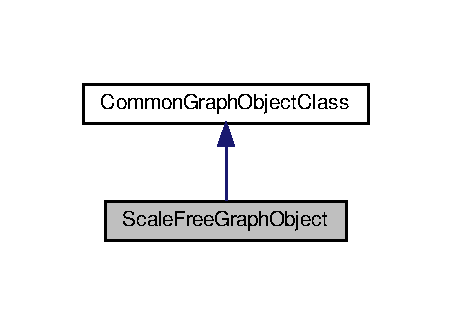
\includegraphics[width=217pt]{classScaleFreeGraphObject__inherit__graph}
\end{center}
\end{figure}


Collaboration diagram for Scale\+Free\+Graph\+Object\+:
\nopagebreak
\begin{figure}[H]
\begin{center}
\leavevmode
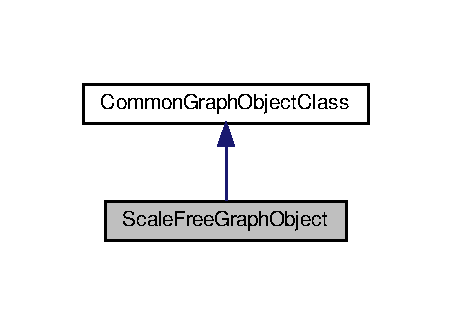
\includegraphics[width=217pt]{classScaleFreeGraphObject__coll__graph}
\end{center}
\end{figure}
\subsection*{Public Types}
\begin{DoxyCompactItemize}
\item 
\mbox{\Hypertarget{classScaleFreeGraphObject_a1f93c4d2a33127b8a87b2a6e05a65887}\label{classScaleFreeGraphObject_a1f93c4d2a33127b8a87b2a6e05a65887}} 
typedef boost\+::plod\+\_\+iterator$<$ boost\+::minstd\+\_\+rand, Graph $>$ {\bfseries S\+F\+Gen}
\end{DoxyCompactItemize}
\subsection*{Public Member Functions}
\begin{DoxyCompactItemize}
\item 
\mbox{\Hypertarget{classScaleFreeGraphObject_aabfcbf560a4154b2132b385fe9d76e2b}\label{classScaleFreeGraphObject_aabfcbf560a4154b2132b385fe9d76e2b}} 
{\bfseries Scale\+Free\+Graph\+Object} (unsigned long num\+\_\+nodes, double A, double B)
\item 
\mbox{\Hypertarget{classScaleFreeGraphObject_ae45db0e0a2a87c7a8f7c06d0da2b02ab}\label{classScaleFreeGraphObject_ae45db0e0a2a87c7a8f7c06d0da2b02ab}} 
void {\bfseries build} ()
\end{DoxyCompactItemize}
\subsection*{Public Attributes}
\begin{DoxyCompactItemize}
\item 
\mbox{\Hypertarget{classScaleFreeGraphObject_a4c692efd6288d5550efc485d3c977a2d}\label{classScaleFreeGraphObject_a4c692efd6288d5550efc485d3c977a2d}} 
unsigned long {\bfseries N}
\item 
\mbox{\Hypertarget{classScaleFreeGraphObject_ae308484fcb176ee722d780b8ac746523}\label{classScaleFreeGraphObject_ae308484fcb176ee722d780b8ac746523}} 
unsigned long {\bfseries E}
\item 
\mbox{\Hypertarget{classScaleFreeGraphObject_a028a9a080967563fc817d69315d1dac5}\label{classScaleFreeGraphObject_a028a9a080967563fc817d69315d1dac5}} 
Graph {\bfseries g}
\item 
\mbox{\Hypertarget{classScaleFreeGraphObject_a5088520127236e2b2be8d7562d8d7dbc}\label{classScaleFreeGraphObject_a5088520127236e2b2be8d7562d8d7dbc}} 
boost\+::minstd\+\_\+rand {\bfseries gen}
\item 
\mbox{\Hypertarget{classScaleFreeGraphObject_a0526d8a58e827cb697c9620674eaf679}\label{classScaleFreeGraphObject_a0526d8a58e827cb697c9620674eaf679}} 
double {\bfseries alpha}
\item 
\mbox{\Hypertarget{classScaleFreeGraphObject_a984fff771258c24b7620c6e946355135}\label{classScaleFreeGraphObject_a984fff771258c24b7620c6e946355135}} 
double {\bfseries beta}
\item 
\mbox{\Hypertarget{classScaleFreeGraphObject_aad974e5ca047974d16d886662c2b06ee}\label{classScaleFreeGraphObject_aad974e5ca047974d16d886662c2b06ee}} 
unsigned long {\bfseries Procs} = num\+\_\+processes(boost\+::graph\+::distributed\+::mpi\+\_\+process\+\_\+group())
\end{DoxyCompactItemize}


The documentation for this class was generated from the following file\+:\begin{DoxyCompactItemize}
\item 
Graph\+Classes/Scale\+Free\+Graph.\+h\end{DoxyCompactItemize}

\hypertarget{classSmallWorldGraphObject}{}\section{Small\+World\+Graph\+Object Class Reference}
\label{classSmallWorldGraphObject}\index{Small\+World\+Graph\+Object@{Small\+World\+Graph\+Object}}


Inheritance diagram for Small\+World\+Graph\+Object\+:
\nopagebreak
\begin{figure}[H]
\begin{center}
\leavevmode
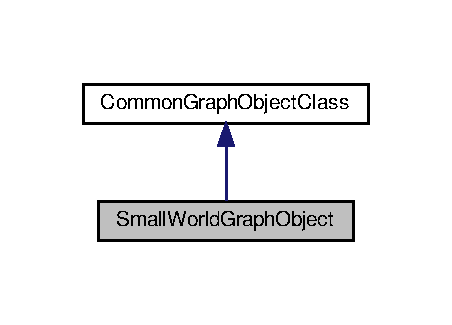
\includegraphics[width=217pt]{classSmallWorldGraphObject__inherit__graph}
\end{center}
\end{figure}


Collaboration diagram for Small\+World\+Graph\+Object\+:
\nopagebreak
\begin{figure}[H]
\begin{center}
\leavevmode
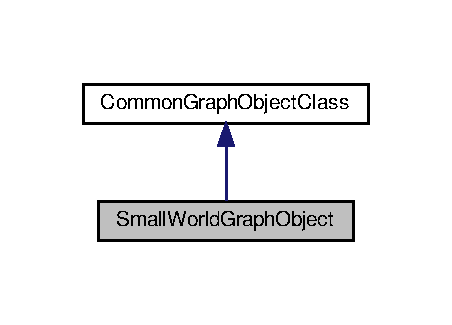
\includegraphics[width=217pt]{classSmallWorldGraphObject__coll__graph}
\end{center}
\end{figure}
\subsection*{Public Types}
\begin{DoxyCompactItemize}
\item 
\mbox{\Hypertarget{classSmallWorldGraphObject_acb009e184bb1bee17aef9cbc5b3e3793}\label{classSmallWorldGraphObject_acb009e184bb1bee17aef9cbc5b3e3793}} 
typedef boost\+::small\+\_\+world\+\_\+iterator$<$ boost\+::minstd\+\_\+rand, Graph $>$ {\bfseries S\+W\+Gen}
\end{DoxyCompactItemize}
\subsection*{Public Member Functions}
\begin{DoxyCompactItemize}
\item 
\mbox{\Hypertarget{classSmallWorldGraphObject_a3cd1132183588dfffba4b6892264f7c9}\label{classSmallWorldGraphObject_a3cd1132183588dfffba4b6892264f7c9}} 
{\bfseries Small\+World\+Graph\+Object} (unsigned long num\+\_\+nodes, unsigned long k\+Neighbors, double probability)
\item 
\mbox{\Hypertarget{classSmallWorldGraphObject_a88b6e629b8058a219a75b1a3eb3ace78}\label{classSmallWorldGraphObject_a88b6e629b8058a219a75b1a3eb3ace78}} 
void {\bfseries build} ()
\end{DoxyCompactItemize}
\subsection*{Public Attributes}
\begin{DoxyCompactItemize}
\item 
\mbox{\Hypertarget{classSmallWorldGraphObject_ac71676e3d70169b86efe9eb8026f22dd}\label{classSmallWorldGraphObject_ac71676e3d70169b86efe9eb8026f22dd}} 
unsigned long {\bfseries N}
\item 
\mbox{\Hypertarget{classSmallWorldGraphObject_ae8743f503dc950297bddc0fe0d479d01}\label{classSmallWorldGraphObject_ae8743f503dc950297bddc0fe0d479d01}} 
unsigned long {\bfseries E}
\item 
\mbox{\Hypertarget{classSmallWorldGraphObject_a93c81ac9467a03d50acf4f652300ee21}\label{classSmallWorldGraphObject_a93c81ac9467a03d50acf4f652300ee21}} 
Graph {\bfseries g}
\item 
\mbox{\Hypertarget{classSmallWorldGraphObject_a2cdff89afdd0a03423557ddb4cb61791}\label{classSmallWorldGraphObject_a2cdff89afdd0a03423557ddb4cb61791}} 
boost\+::minstd\+\_\+rand {\bfseries gen}
\item 
\mbox{\Hypertarget{classSmallWorldGraphObject_a064764c41a03f67791e76d5b957facc0}\label{classSmallWorldGraphObject_a064764c41a03f67791e76d5b957facc0}} 
unsigned long {\bfseries K}
\item 
\mbox{\Hypertarget{classSmallWorldGraphObject_adf39fde9b34c52489a0606c71f071c21}\label{classSmallWorldGraphObject_adf39fde9b34c52489a0606c71f071c21}} 
double {\bfseries Proba}
\item 
\mbox{\Hypertarget{classSmallWorldGraphObject_acd7c02cb7511fe6cd844c10457ff4707}\label{classSmallWorldGraphObject_acd7c02cb7511fe6cd844c10457ff4707}} 
unsigned long {\bfseries Procs} = num\+\_\+processes(boost\+::graph\+::distributed\+::mpi\+\_\+process\+\_\+group())
\end{DoxyCompactItemize}


The documentation for this class was generated from the following file\+:\begin{DoxyCompactItemize}
\item 
Graph\+Classes/Small\+World\+Graph.\+h\end{DoxyCompactItemize}

\hypertarget{structSolverConfig}{}\section{Solver\+Config Struct Reference}
\label{structSolverConfig}\index{Solver\+Config@{Solver\+Config}}
\subsection*{Public Attributes}
\begin{DoxyCompactItemize}
\item 
\mbox{\Hypertarget{structSolverConfig_a48ff380d0d66cd704e86510b5cd3085f}\label{structSolverConfig_a48ff380d0d66cd704e86510b5cd3085f}} 
int {\bfseries s} =0
\item 
\mbox{\Hypertarget{structSolverConfig_a36835c55d433deabaaeaf2135331cf03}\label{structSolverConfig_a36835c55d433deabaaeaf2135331cf03}} 
int {\bfseries d} =0
\item 
\mbox{\Hypertarget{structSolverConfig_aeb7c8b3bf49aaa6e0f365de69808ae10}\label{structSolverConfig_aeb7c8b3bf49aaa6e0f365de69808ae10}} 
double {\bfseries P} \mbox{[}4\mbox{]}
\end{DoxyCompactItemize}


The documentation for this struct was generated from the following files\+:\begin{DoxyCompactItemize}
\item 
Solvers/General\+Solver.\+h\item 
Solvers/General\+Solver.\+cpp\end{DoxyCompactItemize}

\hypertarget{structTimeStructure}{}\section{Time\+Structure Struct Reference}
\label{structTimeStructure}\index{Time\+Structure@{Time\+Structure}}
\subsection*{Public Attributes}
\begin{DoxyCompactItemize}
\item 
\mbox{\Hypertarget{structTimeStructure_affed43a1754e3d3825115e62431e3d43}\label{structTimeStructure_affed43a1754e3d3825115e62431e3d43}} 
double {\bfseries h} = 0.\+01
\item 
\mbox{\Hypertarget{structTimeStructure_a15205e0ecbe3c3c176c838ad4a1e1028}\label{structTimeStructure_a15205e0ecbe3c3c176c838ad4a1e1028}} 
double {\bfseries t} = 0
\end{DoxyCompactItemize}


The documentation for this struct was generated from the following file\+:\begin{DoxyCompactItemize}
\item 
Solvers/General\+Solver.\+h\end{DoxyCompactItemize}

%--- End generated contents ---

% Index
\backmatter
\newpage
\phantomsection
\clearemptydoublepage
\addcontentsline{toc}{chapter}{Index}
\printindex

\end{document}
